% Copyright 2004 by Till Tantau <tantau@users.sourceforge.net>.
%
% In principle, this file can be redistributed and/or modified under
% the terms of the GNU Public License, version 2.
%
% However, this file is supposed to be a template to be modified
% for your own needs. For this reason, if you use this file as a
% template and not specifically distribute it as part of a another
% package/program, I grant the extra permission to freely copy and
% modify this file as you see fit and even to delete this copyright
% notice.

\documentclass{beamer}

\usepackage{tikz}
\usetikzlibrary{automata, matrix,shapes.multipart,shapes.geometric,fit,scopes,positioning}

\definecolor{blue-base}{RGB}{42, 79, 110}
\definecolor{purple-custom}{RGB}{54, 51, 119}
\definecolor{orange-custom}{RGB}{227, 164, 79}
\definecolor{yellow-custom}{RGB}{170, 142, 57}

% There are many different themes available for Beamer. A comprehensive
% list with examples is given here:
% http://deic.uab.es/~iblanes/beamer_gallery/index_by_theme.html
% You can uncomment the themes below if you would like to use a different
% one:
%\usetheme{AnnArbor}
%\usetheme{Antibes}
%\usetheme{Bergen}
%\usetheme{Berkeley}
%\usetheme{Berlin}
%\usetheme{Boadilla}
%\usetheme{boxes}
%\usetheme{CambridgeUS}
%\usetheme{Copenhagen}
%\usetheme{Darmstadt}
%\usetheme{default}
%\usetheme{Frankfurt}
%\usetheme{Goettingen}
%\usetheme{Hannover}
%\usetheme{Ilmenau}
%\usetheme{JuanLesPins}
%\usetheme{Luebeck}
\usetheme{Madrid}
%\usetheme{Malmoe}
%\usetheme{Marburg}
%\usetheme{Montpellier}
%\usetheme{PaloAlto}
%\usetheme{Pittsburgh}
%\usetheme{Rochester}
%\usetheme{Singapore}
%\usetheme{Szeged}
%\usetheme{Warsaw}

\title{ADT PLM}

% A subtitle is optional and this may be deleted
\subtitle{Programmer's Learning Machine}

\author{Matthieu~Nicolas}

\date{IJD Seminar, 2016-02-02}

\subject{Theoretical Computer Science}

\AtBeginSection[]
{
  \begin{frame}<beamer>{Outline}
    \tableofcontents[currentsection]
  \end{frame}
}

\begin{document}

\begin{frame}
  \titlepage
\end{frame}

\begin{frame}{Outline}
  \tableofcontents
  % You might wish to add the option [pausesections]
\end{frame}

\section{Presentation of PLM}

\subsection{Purposes}

\begin{frame}{Presentation of PLM}{Purposes}
  \begin{itemize}
  \item {
    Application to learn programming.
    \pause
  }
  \item {
    Allows students to progress at their own speed...
    \pause
  }
  \item {
    ... while the teacher helps the ones having trouble.
    \pause
  }
  \item {
    Used at TELECOM Nancy since 2008.
  }
  \end{itemize}
\end{frame}

\subsection{Demo}

% TODO: Record the video
\begin{frame}{Presentation of PLM}{Quick demo}
  \begin{center}
    \href{https://plm.telecomnancy.univ-lorraine.fr}{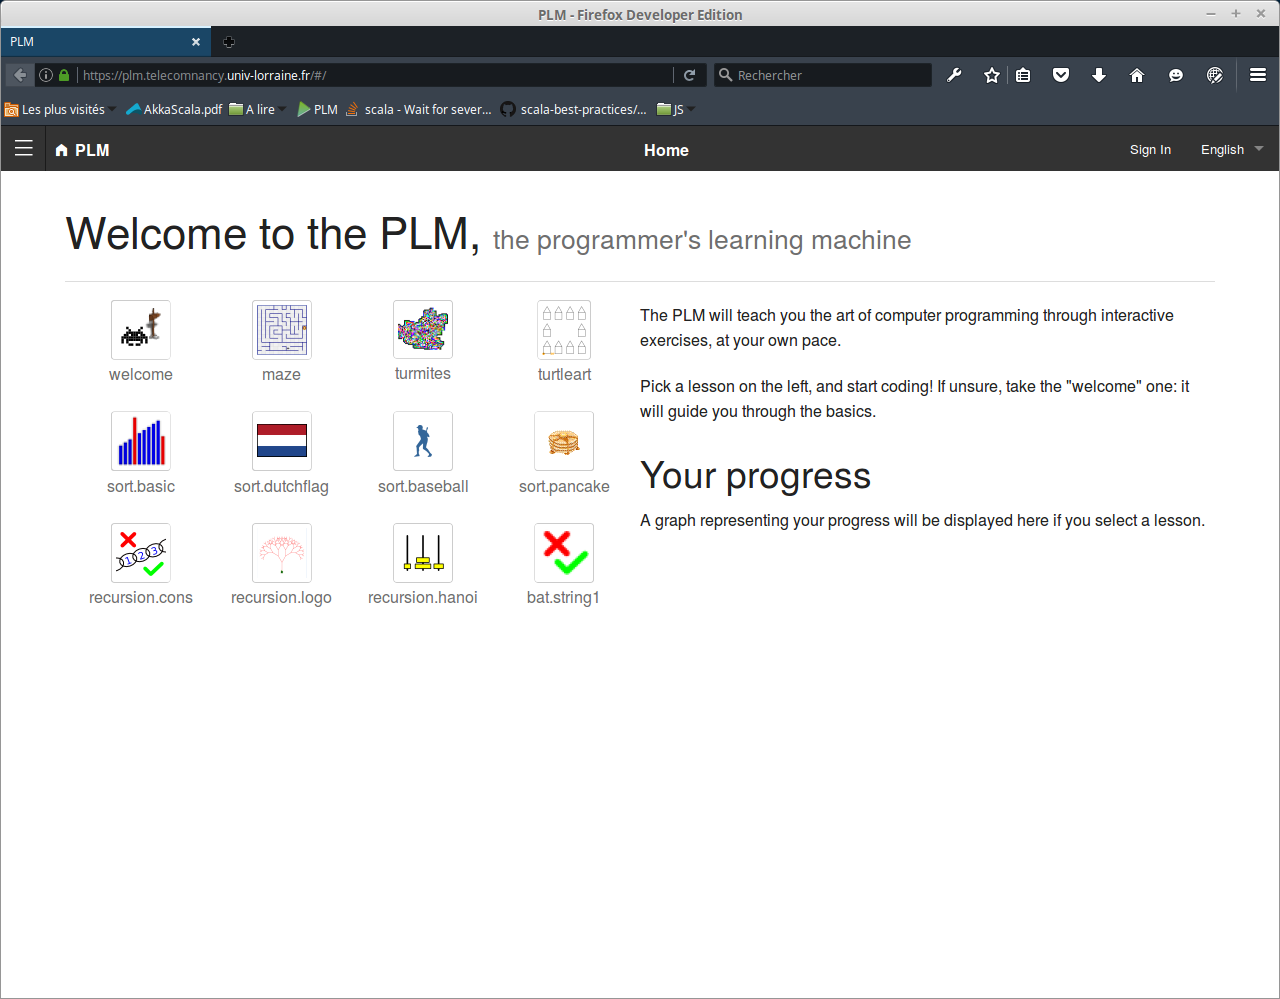
\includegraphics[scale=0.16]{img/screen-webPLM-1.png}}
    \begin{itemize}
    \item Available at \url{https://plm.telecomnancy.univ-lorraine.fr}
    \end{itemize}
  \end{center}
\end{frame}

\subsection{About PLM}

% QUESTION: Need slides for these infos or talk about them in the video?
\begin{frame}{Presentation of PLM}{12 lessons, 200 exercises}
  \begin{center}
    \includegraphics[scale=0.18]<1>{img/maze.png}
    \includegraphics[scale=0.18]<2>{img/hanoi.png}
    \includegraphics[scale=0.18]<3>{img/logo.png}
  \end{center}
\end{frame}

\begin{frame}{Presentation of PLM}{Languages and programming languages}
  \begin{itemize}
    \item {
      Available languages:
      \begin{itemize}
      \item English
      \item French
      \item Brazilian Portuguese
      \end{itemize}
    }
    \item[~]
    \item {
      Supported programming languages:
    }
  \end{itemize}
  \begin{center}
    
\includegraphics[scale=0.16]{img/java.png}
    ~
    
\includegraphics[scale=0.4]{img/scala.png}
    
\includegraphics[scale=0.18]{img/python.png}
  \end{center}
\end{frame}

\subsection{Architecture}

\begin{frame}{Presentation of PLM}{Application's architecture}
  \begin{center}
    \begin{tikzpicture}[
      scale=1,
      block/.style={
        rectangle, rounded corners=9pt,
        text width=8em,
        text centered,
        minimum height=3em,
        draw=black!50,
        fill=black!20
      },
      oauth/.style={
        block,
        color=white,
        fill=purple-custom
      }
    ]

      \node (user) { 
\includegraphics[scale=0.05]{img/user.pdf} };

      \node[block, right=1.5 of user, align=center] (webPLM) {webPLM\\(centralized/local)};

      \node[block, right=1.5 of webPLM] (plm-data) { PLM-data };

      % OAuth-providers
      \node[oauth, scale=0.5, below=1.5 of user] (plm-accounts) { PLM-accounts };
      \node[scale=0.5, below=0.3 of plm-accounts] (google) { 
\includegraphics[scale=0.1]{img/google-logo.png} };
      \node[scale=0.5, below=0.3 of google] (github) { 
\includegraphics[scale=0.1]{img/github-logo.png} };
      \node[draw=purple-custom, densely dotted, fit=(plm-accounts) (google) (github)] (oauth-providers) {};
      \node[color=purple-custom, below=0.1 of oauth-providers] {OAuth-providers};

      \node[block, below=2.5 of plm-data] (plm-profiles) { PLM-profiles };

      \path[<->, shorten >=3pt, shorten <=3pt]
        (user) edge (webPLM)
        (user) edge node[left, scale=0.6] {authentificate} (oauth-providers)
        (webPLM) edge (plm-data)
        (webPLM) edge[bend right] node[above right, align=center, xshift=-5, scale=0.6] {retrieve user's \\ preferences} (plm-profiles.west)
        (webPLM) edge[bend left] node[below right, align=center, yshift=-15, xshift=-25, scale=0.6]  {validate \\ authentification} (oauth-providers.east);

    \end{tikzpicture}
  \end{center}
\end{frame}

\section{To a web app}

\subsection{Goals}

\begin{frame}{To a web app}{Evolution of the project}
  \begin{itemize}
    \item {
      Formerly a fat client
      \begin{itemize}
        \item { Written in Java }
      \end{itemize}
      \pause
    }
    \item[~]
    \item {
      Switch to a web application
      \begin{itemize}
        \item { Server implemented in Scala using \emph{PlayFramework} }
        \item { User interface written in Javascript using \emph{AngularJS} and \emph{Foundation} }
      \end{itemize}
    }
  \end{itemize}
  \begin{center}
    
\includegraphics[scale=0.05]{img/play-logo.png}
    ~
    
\includegraphics[scale=0.1]{img/foundation-angular.png}
  \end{center}
\end{frame}

% TODO: Complete slide and find a better title
% Add item about making it easier to access to PLM and to try it
\begin{frame}{To a web app}{Motivations}
  \begin{itemize}
  \item {
    More user-friendly
  }
  \item {
    Aim to setup SPOC\footnote{Small Private Online Course} and MOOC\footnote{Massive Open Online Course}
  }
  \item[~]
  \item {
    But don't have the time and means for a reboot
  }
  \end{itemize}
\end{frame}

\subsection{PLM as a library}

% TODO: Add schema of PLM's components
\begin{frame}{To a web app}{Refactoring PLM}
  \begin{itemize}
  \item {
    Implemented a headless version of PLM: \emph{PLM-engine}
    \begin{itemize}
    \item Provide all PLM's content and methods
    \item But without a user interface
    \end{itemize}
  }
  \end{itemize}
\end{frame}

\begin{frame}{To a web app}{Implementing the server}
  \begin{itemize}
  \item {
    Designed a communication protocol between the server and the client
    \begin{itemize}
    \item User's actions sent to server as JSON messages
    \end{itemize}
  }
  \item {
    Only need to implement an interpreter
    \begin{itemize}
    \item Parse messages received from the client
    \item Query or command PLM-engine according to the message
    \item Send back result or acknowledgement to the client
    \end{itemize}
  }
  \end{itemize}
\end{frame}

\subsection{Outcome}

\begin{frame}{To a web app}{Interactions between components}
  \begin{center}
    % QUESTION: how to picture it better?
    % Go further in details?
    \begin{tikzpicture}[
      scale=1,
      block/.style={
        rectangle, rounded corners=9pt,
        text width=8em,
        text centered,
        minimum height=3em,
        draw=black!50,
        fill=black!20
      }
    ]

      \node (user) { 
\includegraphics[scale=0.05]{img/user.pdf} };

      \node[block, right=2 of user] (plm-actor) { PLM-actor };
      \node[block, right=2 of plm-actor] (plm-engine) { PLM-engine };

      \node[draw, densely dotted, fit=(plm-actor) (plm-engine)] (webPLM) {};
      \node[below=0.1 of webPLM] {webPLM};

      \path[->, shorten >=2pt, shorten <=2pt]
        (user) edge node[sloped, anchor=center, above] {\tiny user's action} (plm-actor)
        (plm-actor) edge node[sloped, anchor=center, above] {\tiny query / command} (plm-engine)
        ([yshift=-0.2 cm]plm-engine.west) edge node[sloped, anchor=center, below] {\tiny send result} ([yshift=-0.2 cm]plm-actor.east)
        ([yshift=-0.2 cm]plm-actor.west) edge node[sloped, anchor=center, below] {\tiny relay result} ([yshift=-0.2 cm]user.east);
    \end{tikzpicture}
  \end{center}
\end{frame}

% TODO: Find a better subtitle
% TODO: Complete this slide
\begin{frame}{To a web app}{Results}
  \begin{itemize}
  \item {
    Build quickly a web application from the fat client...
  }
  \item {
    ... but can't share common ressources among users
  }
  \end{itemize}
\end{frame}

\section{Assessment of user's code}

\subsection{Challenges}

\begin{frame}{Assessment of user's code}{Limits}
  \begin{itemize}
  \item {
    Run on the same machine, same JVM
    \pause
  }
  \item[~]
  \item {
    How to protect ourselves from users' rookie mistakes?
    \begin{itemize}
    \item {
      Infinite loops
    }
    \end{itemize}
    \pause
  }
  \item {
    And from more malicious "mistakes"?
    \begin{itemize}
    \item {
      Infinite thread creation
    }
    \item {
      Endless file creation
    }
    \end{itemize}
    \pause
  }
  \item {
    And from \emph{System.exit(whatever)}?
    \pause
  }
  \item[~]
  \item {
    Scalability issues
  }
  \end{itemize}
\end{frame}

\subsection{Extraction of the execution component}

\begin{frame}{Assessment of user's code}{Delegate execution to workers}
  \begin{itemize}
  \item Called \emph{Judges} in the litterature
  \item Use PLM-engine as well
  \item[~]
  \item {
    Workflow:
    \begin{itemize}
    \item Retrieve an execution request
    \item Parse the request to extract parameters
    \item Configure PLM-engine according to them
    \item Run the user's code
    \item Send back result to webPLM
    \end{itemize}
  }
  \end{itemize}
\end{frame}

% TODO: Describe message queue
\begin{frame}{Assessment of user's code}{Message queues}
  \begin{itemize}
    \item {
      Message-driven architecture
    }
    % TODO: "Découplage des composants"
    \item {
      Help to implement:
      \begin{itemize}
        \item Producer/Consumer pattern
        \item \alert<2> {Request/Response pattern}
      \end{itemize}
    }
    \item {
      % TODO: Rephrase
      Different reliability patterns of the message processing:
      \begin{itemize}
        \item \alert<2> {Only one worker}
        \item At least one worker
        \item All workers
      \end{itemize}
    }
  \end{itemize}
\end{frame}

\begin{frame}{Assessment of user's code}{Architecture with judges}
  \begin{center}
    \begin{tikzpicture}[
      scale=1,
      block/.style={
        rectangle, rounded corners=9pt,
        text width=8em,
        text centered,
        minimum height=3em,
        draw=black!50,
        fill=black!20
      },
      judge/.style={
        block,
        text width=4em
      }
    ]

      \node (user) { 
\includegraphics[scale=0.05]{img/user.pdf} };

      \node[block, right=3 of user] (plm-actor) { PLM-actor };
      \node[block, right=1 of plm-actor] (plm-engine) { PLM-engine };

      \node[draw, densely dotted, fit=(plm-actor) (plm-engine)] {};
      \node[fit=(plm-actor) (plm-engine), yshift=-30, xshift=30] {webPLM};

      \node[below=1.5 of plm-actor] (center-mq) {};

      \node[right=0.05 of center-mq] (requests-mq) { 
\includegraphics[angle=-90, scale=0.3]{img/message-queue-2.png} };
      \node[right=0.05 of center-mq, xshift=20] {\tiny \textbf{Requests}};

      \node[left=0.05 of center-mq] (reply-mq) { 
\includegraphics[angle=90, scale=0.3]{img/message-queue-2.png} };
      \node[left=0.05 of center-mq, xshift=-20] {\tiny \textbf{Reply}};

      \node[judge, below=1.5 of center-mq] (judge1) {Judge 1};
      \node[judge, right=of judge1] (judge2) {Judge 2};
      \node[right=of judge2] (judge3) {...};

      \node[draw, densely dotted, fit=(judge1) (judge2) (judge3)] {};
      \node[fit=(judge1) (judge2) (judge3), yshift=-35] {Judges};

      \path[->, shorten >=2pt, shorten <=2pt]
        (user) edge node[sloped, anchor=center, above] {\tiny request execution} (plm-actor)
        (plm-actor) edge node[sloped, anchor=center, above] {\tiny save result} (plm-engine)
        ([yshift=-0.2 cm]plm-actor.west) edge node[sloped, anchor=center, below] {\tiny relay results} ([yshift=-0.2 cm]user.east);
      \path[->, shorten >=2pt, shorten <=2pt]
        (plm-actor.south) edge[bend left] node[below right] {\tiny submit request} (requests-mq.north)
        (requests-mq.south) edge[bend left] node[right] {\tiny retrieve request} (judge1.north)
        (judge1.north) edge[bend left] node[left] {\tiny send result} (reply-mq.south)
        (reply-mq.north) edge[bend left] node[left] {\tiny retrieve result} (plm-actor.south);
    \end{tikzpicture}
  \end{center}
\end{frame}

\begin{frame}{Assessment of user's code}{Pros and cons}
  \begin{itemize}
  \item {
    Pros:
    \begin{itemize}
    \item Allow to run code without impacting webPLM's performances
    \item Meet the scalability requirements
    \end{itemize}
    \pause
  }
  \item[~]
  \item {
    Cons:
    \begin{itemize}
    \item Make sure to use the right version of PLM-engine
    \item Need to deploy them easily
    \item Should restart them after each execution
    \item Have to restrict their resources usage
    \end{itemize}
  }
  \end{itemize}
\end{frame}

\subsection{Docker}

\begin{frame}{Assessment of user's code}{Docker}
  \begin{itemize}
  \item {
    Lightweight virtualization tool
  }
  \item {
    Build image of your application
  }
  \item {
    Run containers based on images
  }
  \end{itemize}
  \begin{center}
    
\includegraphics[scale=0.2]{img/docker-logo.png}
  \end{center}
\end{frame}

\begin{frame}{Assessment of user's code}{Example of Dockerfile}
  \begin{itemize}
  \item {
    Dockerfiles describe how to set up the application
  }
  \begin{center}
    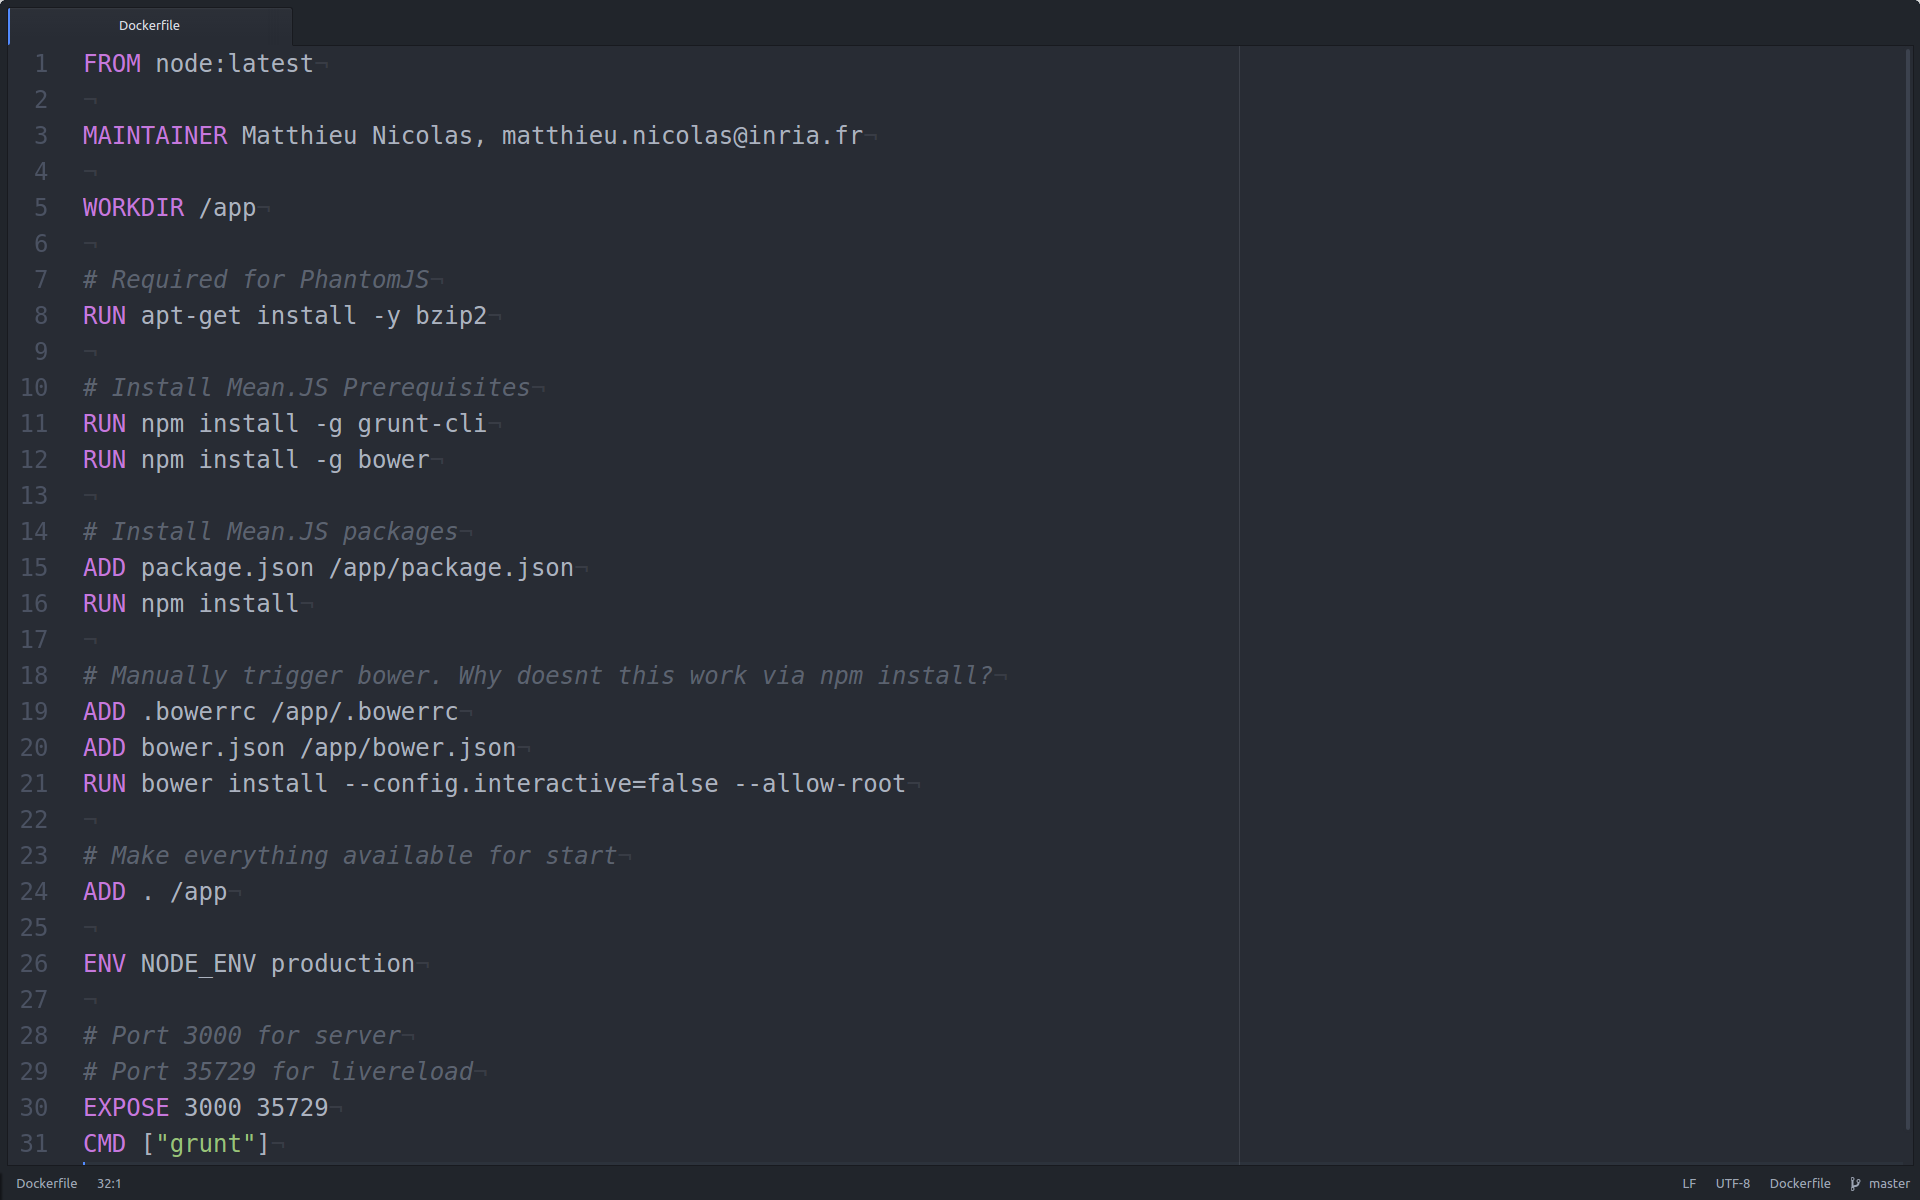
\includegraphics[scale=0.12]{img/dockerfile.png}
  \end{center}
  \item {
    Run \emph{docker build \textcolor{red}{-t tag} \textcolor{blue}{/path/to/Dockerfile}} to build  the image
  }
  \item {
    Start containers with \emph{docker run \textcolor{red}{tag}}
  }
  \end{itemize}
\end{frame}

{ % all template changes are local to this group.
  \setbeamertemplate{navigation symbols}{}
  \begin{frame}[plain]
      \begin{tikzpicture}[remember picture,overlay]
          \node[at=(current page.center)] {
              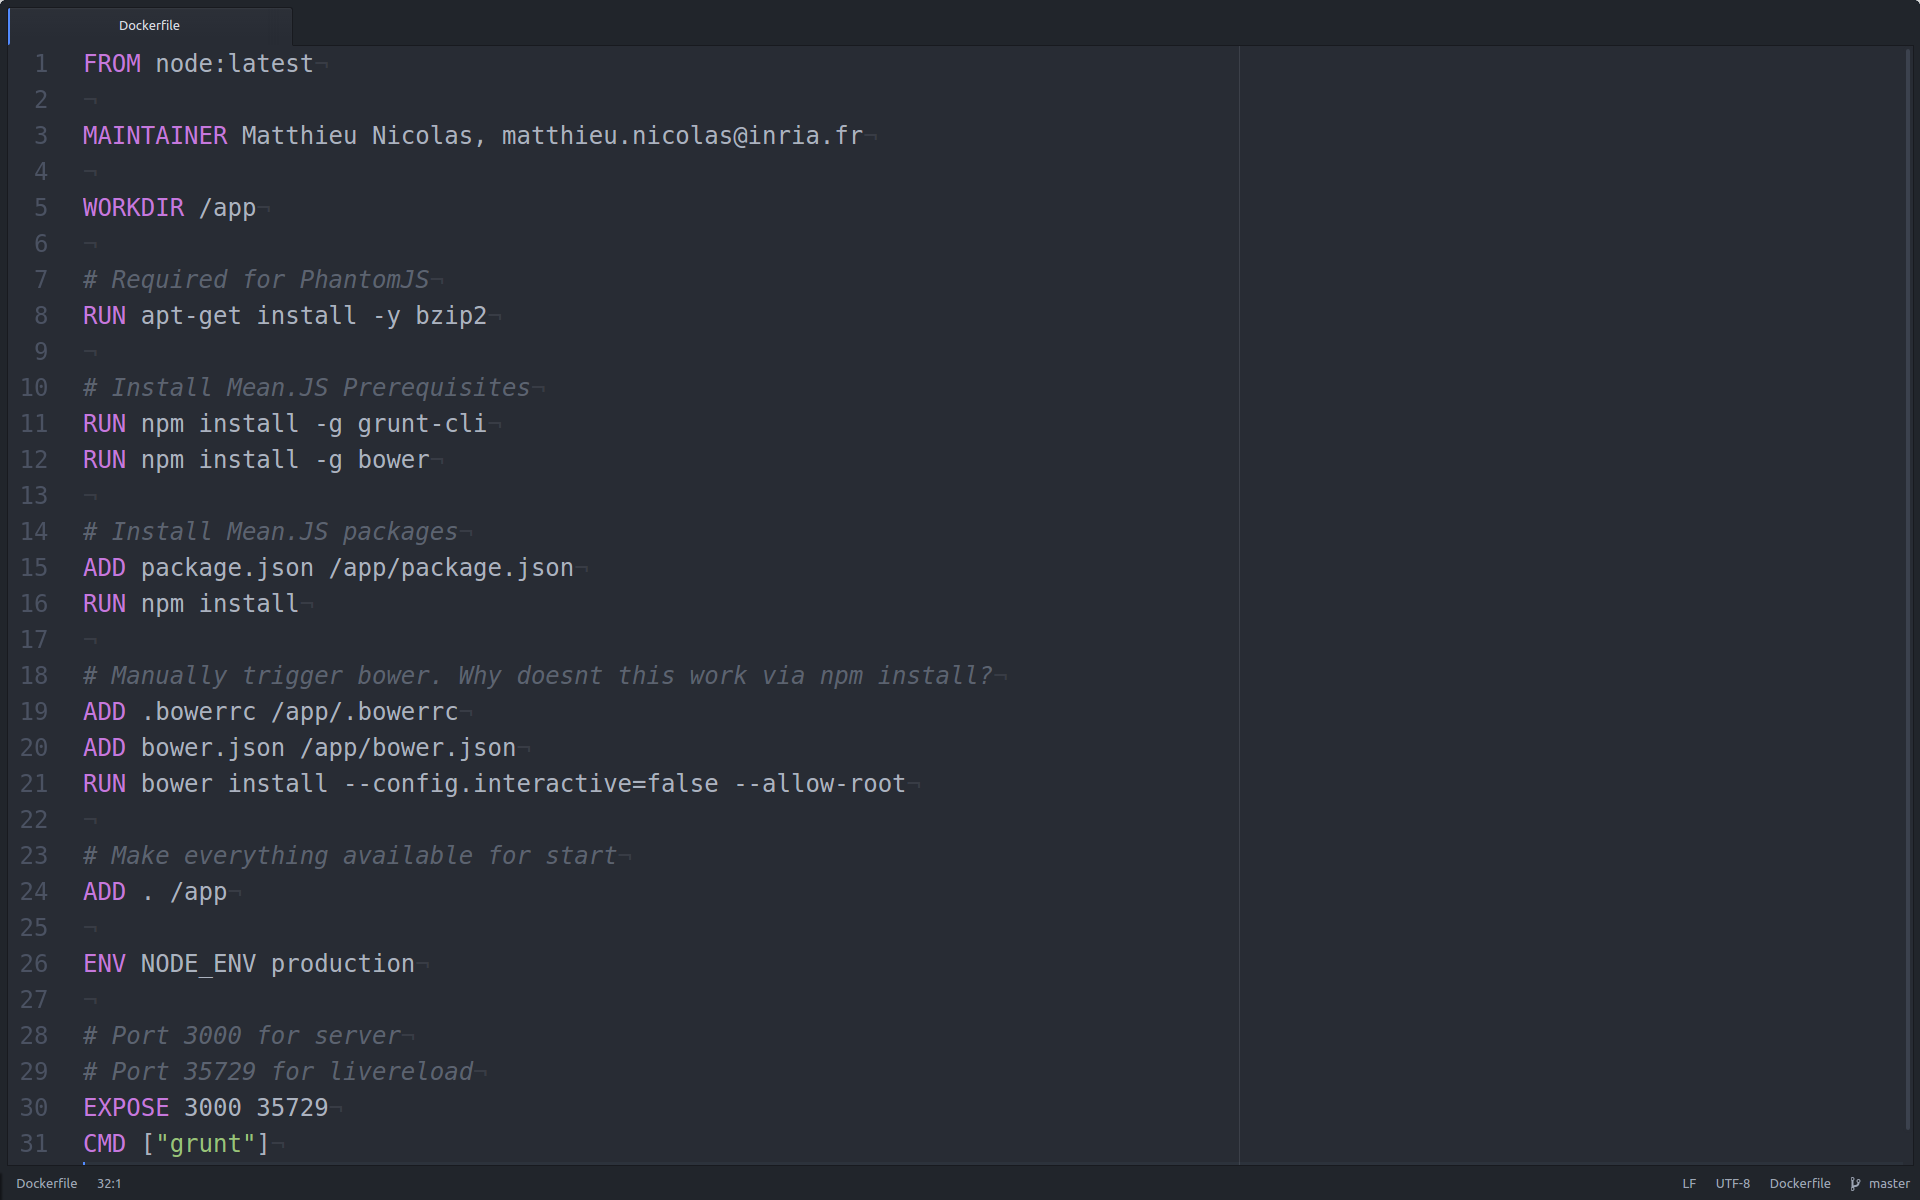
\includegraphics[width=\paperwidth]{img/dockerfile.png}
          };
      \end{tikzpicture}
  \end{frame}
}

\begin{frame}{Assessment of user's code}{Example of Dockerfile}
  \begin{itemize}
  \item {
    Dockerfiles describe how to set up the application
  }
  \begin{center}
    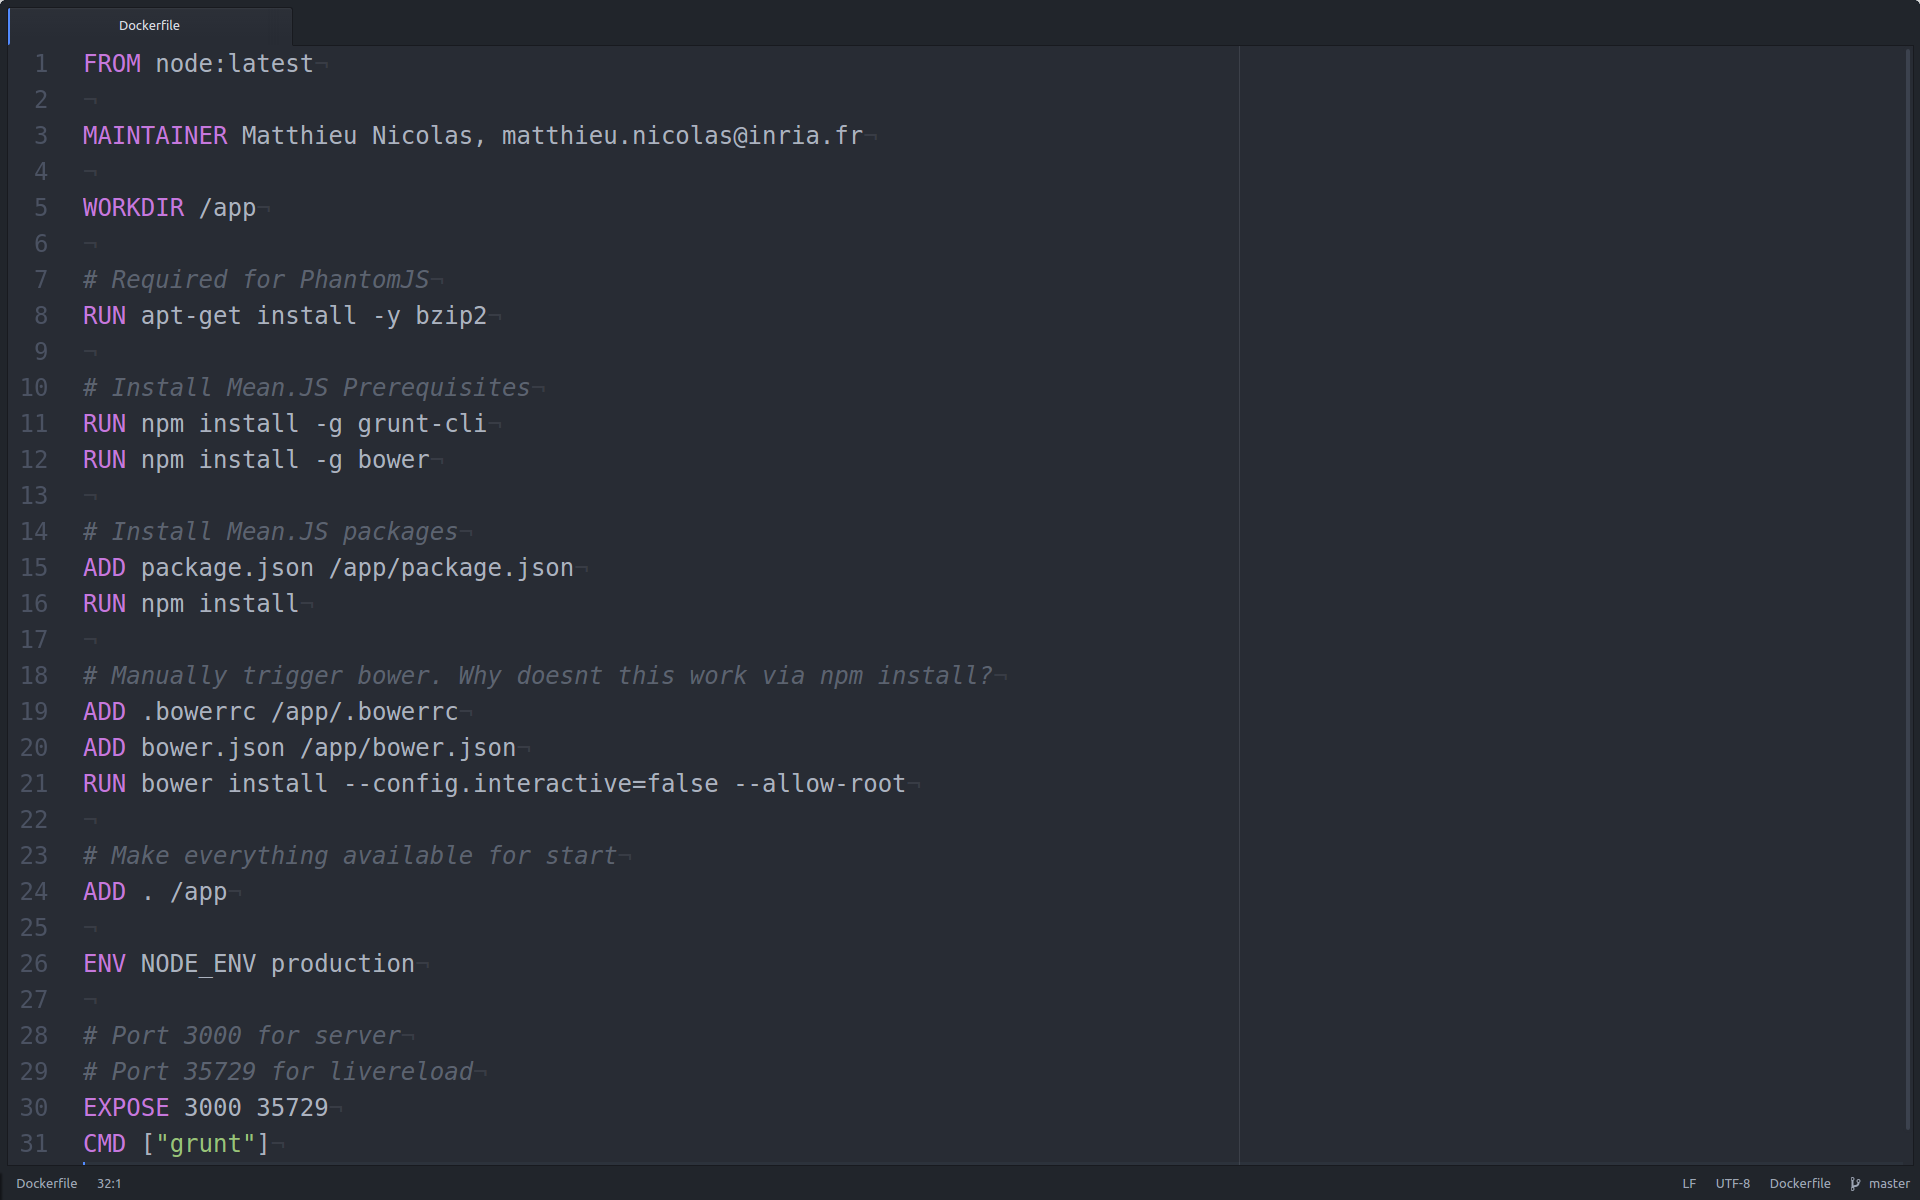
\includegraphics[scale=0.12]{img/dockerfile.png}
  \end{center}
  \item {
    Run \emph{docker build \textcolor{red}{-t tag} \textcolor{blue}{/path/to/Dockerfile}} to build  the image
  }
  \item {
    Start containers with \emph{docker run \textcolor{red}{tag}}
  }
  \end{itemize}
\end{frame}

\begin{frame}{Assessment of user's code}{More about \emph{docker run}}
  \begin{itemize}
  \item {
    Can also manage
    \begin{itemize}
    \item {
      Ports
      \pause
    }
    \item {
      Volumes
      \pause
    }
    \item {
      Links between containers
      \pause
    }
    \item {
      Environment variables
    }
    \item {
      Runtime constraints on resources
    }
    \item {
      Restart policies
    }
    \item {
      And a \textbf{lot more}
      \pause
    }
    \end{itemize}
  }
  \item[~]
  \item {
    Commands can become quite complex
  }
  \end{itemize}
  \begin{center} {
    \emph{docker run \textcolor{blue}{-p 443:9443} \textcolor{red}{-link plm-accounts:accounts} \textcolor{green}{-v \raise.17ex\hbox{$\scriptstyle\sim$}/webPLM/logs/:/app/webplm-dist/logs} webPLM}
  }
  \end{center}
\end{frame}

\begin{frame}{Assessment of user's code}{Docker-compose}
  \begin{itemize}
  \item {
    Tool to easily deploy multi-containers applications
  }
  \begin{center}
    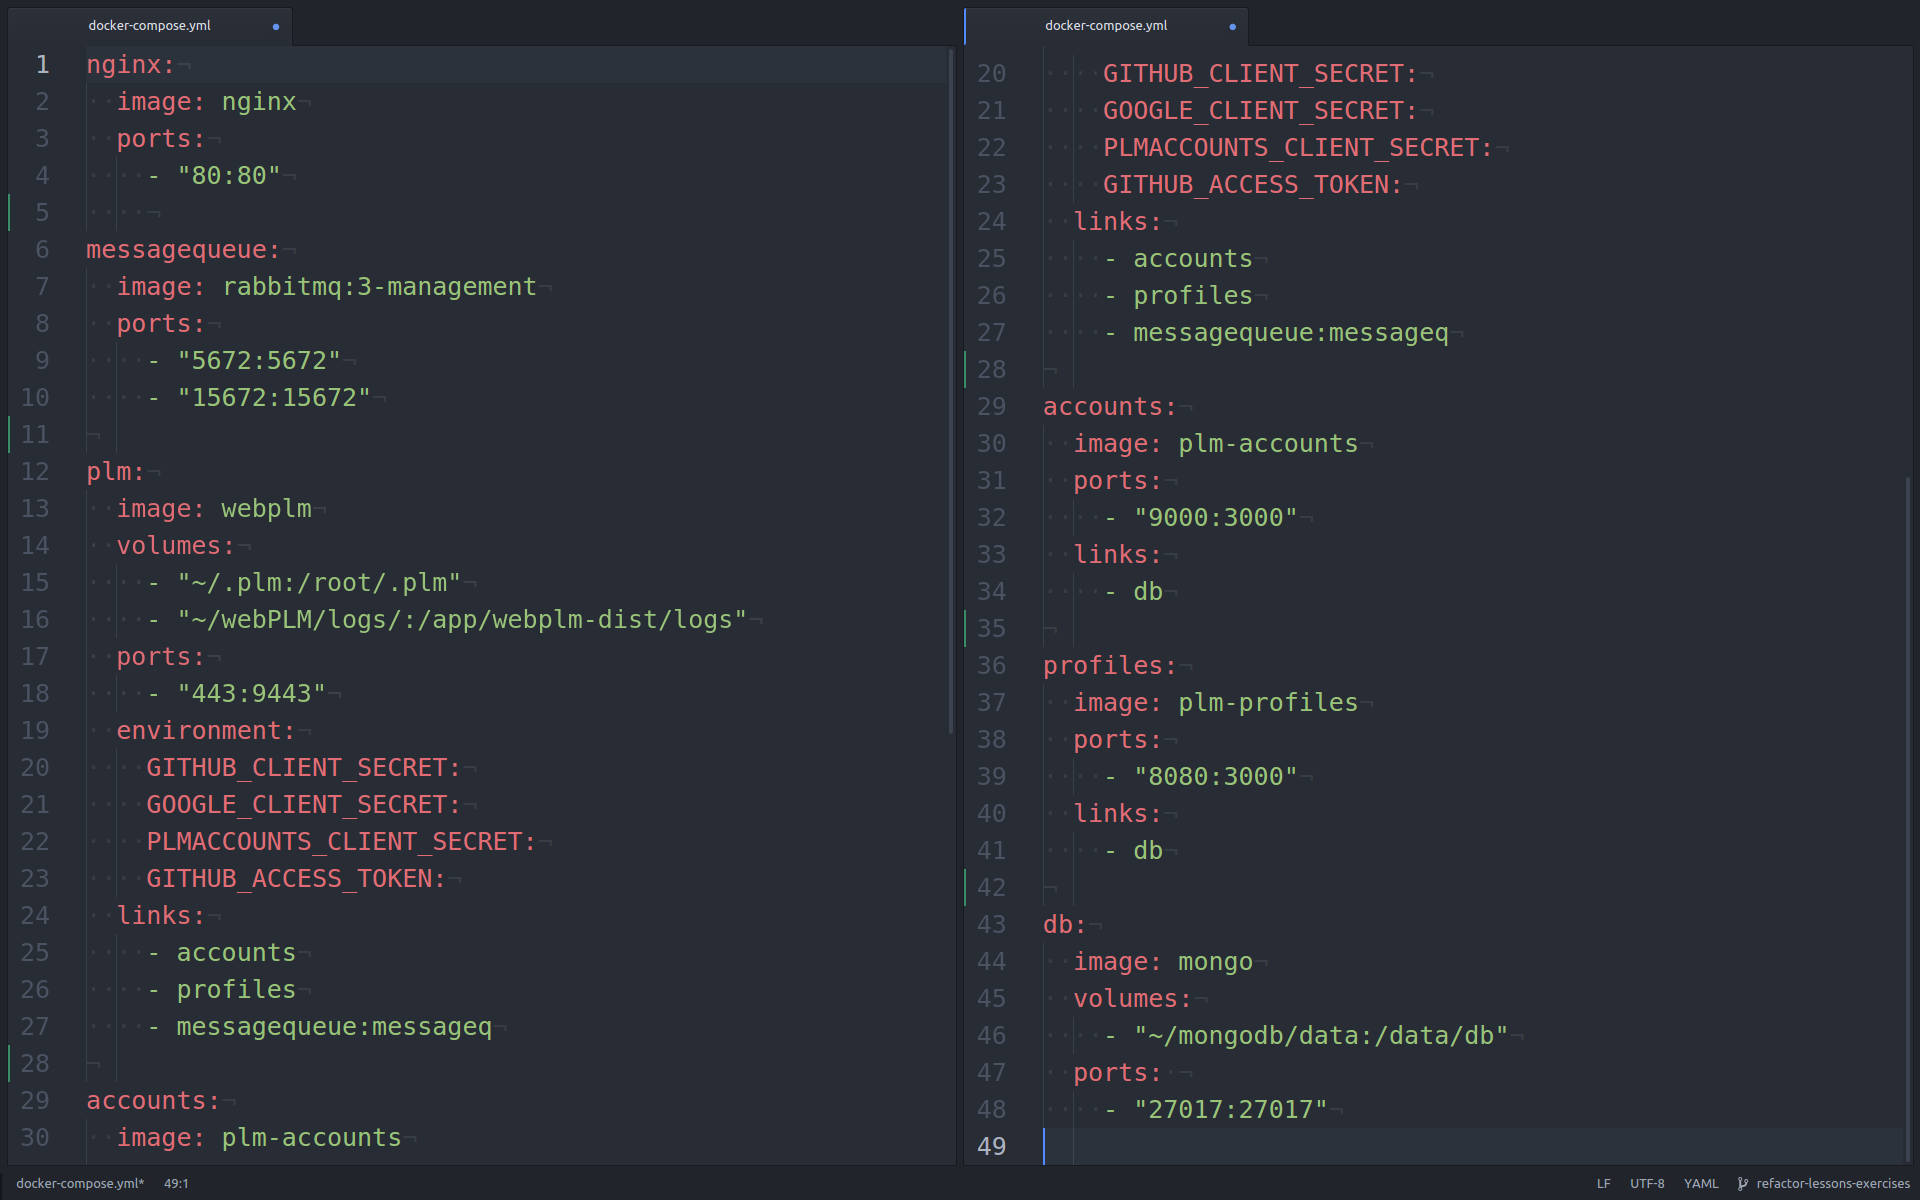
\includegraphics[scale=0.14]{img/docker-compose-2.png}
  \end{center}
  \item {
    Deploy environment with \emph{docker-compose up}
  }
  \end{itemize}
\end{frame}

{ % all template changes are local to this group.
  \setbeamertemplate{navigation symbols}{}
  \begin{frame}[plain]
      \begin{tikzpicture}[remember picture,overlay]
          \node[at=(current page.center)] {
              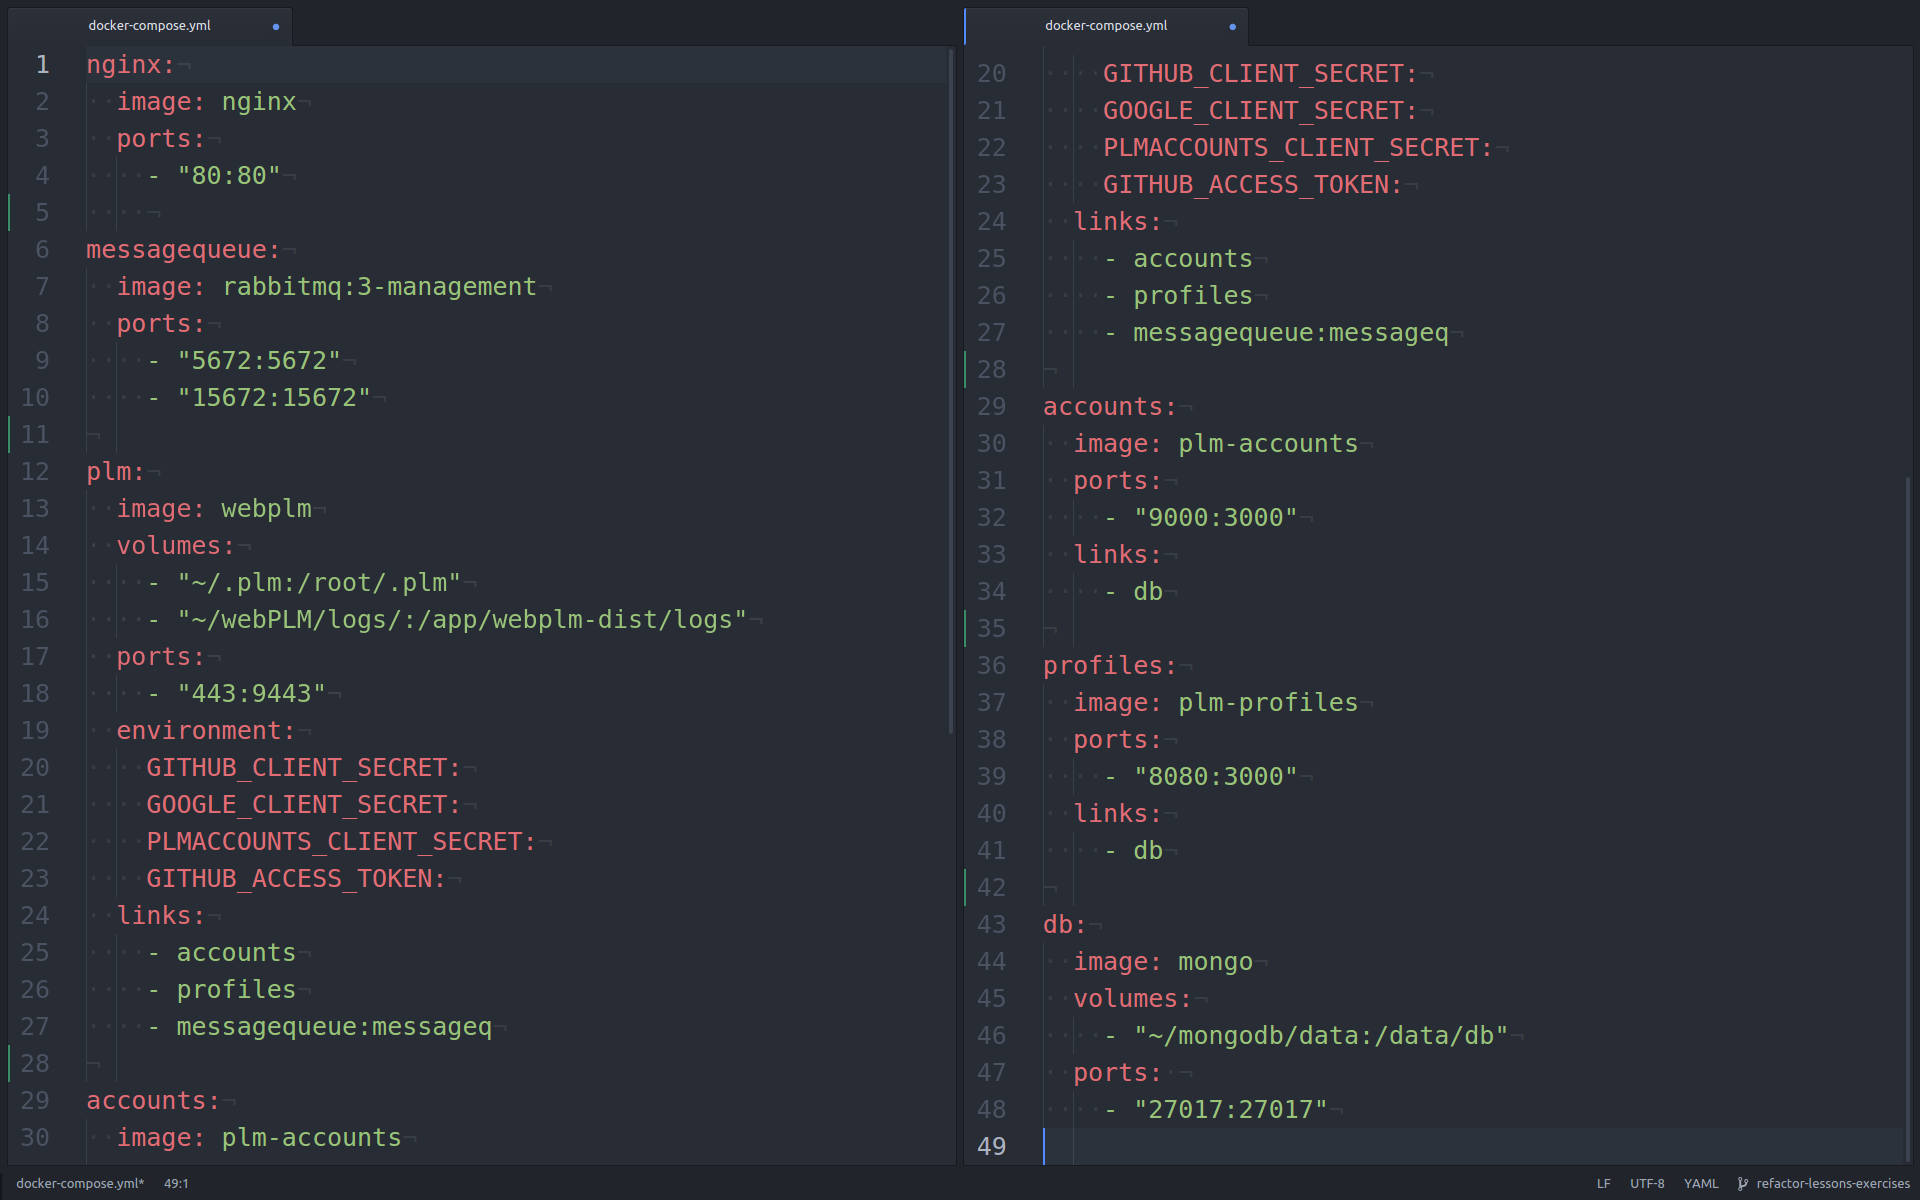
\includegraphics[width=\paperwidth]{img/docker-compose-2.png}
          };
      \end{tikzpicture}
  \end{frame}
}

\begin{frame}{Assessment of user's code}{Docker-compose}
  \begin{itemize}
  \item {
    Tool to easily deploy multi-containers applications
  }
  \begin{center}
    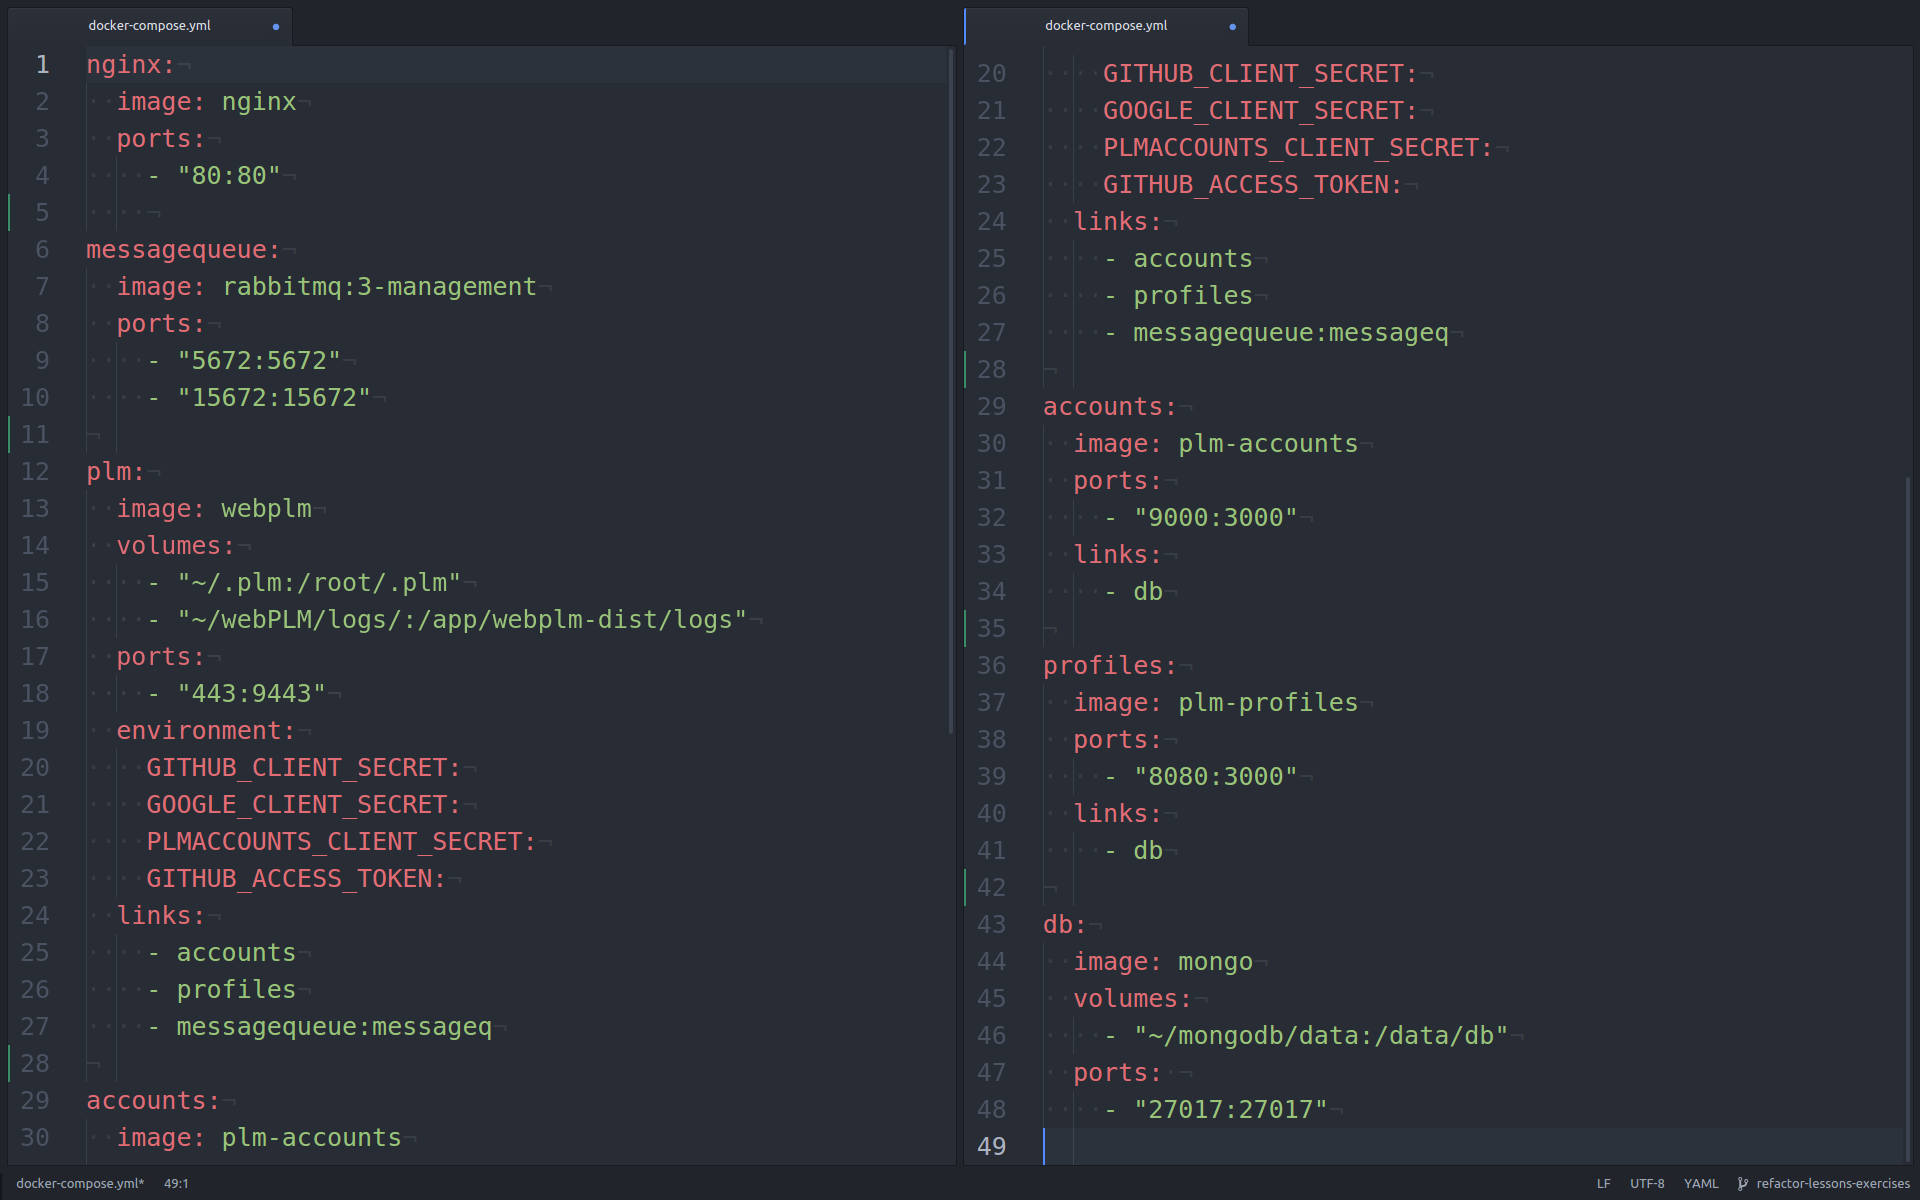
\includegraphics[scale=0.14]{img/docker-compose-2.png}
  \end{center}
  \item {
    Deploy environment with \emph{docker-compose up}
  }
  \end{itemize}
\end{frame}

\begin{frame}{Assessment of user's code}{Docker in our case}
  \begin{itemize}
  \item{
    Deploy easily all components
  }
  \item {
    Restart judges automatically
  }
  \item {
    Limit users' mischiefs
  }
  \end{itemize}
\end{frame}

\section{Result}

\begin{frame}{Result}{Current architecture}
  \begin{center}
    \begin{tikzpicture}[
      scale=1,
      block/.style={
        rectangle, rounded corners=9pt,
        text width=6em,
        text centered,
        minimum height=3em,
        draw=black!50,
        fill=black!20
      },
      oauth/.style={
        block,
        color=white,
        fill=purple-custom
      },
      judge/.style={
        block,
        text width=4em
      }
    ]

      \node (user) { 
\includegraphics[scale=0.05]{img/user.pdf} };
      \node[block, right=of user] (nginx) { nginx };

      %%%%%%%%%%%%%%%%%%
      % webPLMs
      %%%%%%%%%%%%%%%%%%
      %\node[block, above right=of nginx, yshift=-30] (webPLM1) { webPLM-1 };
      %\node[block, below right=of nginx, yshift=30] (webPLM2) { webPLM-2 };
      %\node[draw, densely dotted, fit=(webPLM1) (webPLM2)] {};
      %\node[fit=(webPLM1) (webPLM2)] (webPLMs) {webPLMs};
      \node[block, right=of nginx] (webPLM) {webPLM};

      \path[<->, shorten >=3pt, shorten <=3pt]
        (user) edge (nginx)
        (nginx) edge (webPLM);

      \node[block, right=of webPLM] (plm-data) { PLM-data };
      \node[block, below=0.6 of plm-data] (plm-profiles) { PLM-profiles };

      \path[<->, shorten >=3pt, shorten <=3pt]
        (webPLM) edge (plm-data)
        (webPLM) edge[bend right] (plm-profiles);

      %%%%%%%%%%%%%%%%%%
      % OAuth-providers
      %%%%%%%%%%%%%%%%%%
      \node[oauth, scale=0.5, below=of nginx] (plm-accounts) { PLM-accounts };
      \node[scale=0.5, below=0.3 of plm-accounts] (google) { 
\includegraphics[scale=0.1]{img/google-logo.png} };
      \node[scale=0.5, below=0.3 of google] (github) { 
\includegraphics[scale=0.1]{img/github-logo.png} };
      \node[draw=purple-custom, densely dotted, fit=(plm-accounts) (google) (github)] (oauth-providers) {};
      \node[color=purple-custom, below=0.1 of oauth-providers] {OAuth-providers};

      \path[<->, shorten >=3pt, shorten <=3pt]
        (user) edge[bend right] (oauth-providers)
        (webPLM.south)[xshift=-10] edge[bend left] (oauth-providers.east);

      %%%%%%%%%%%%%%%%%%
      % Judges
      %%%%%%%%%%%%%%%%%%
      \node[below right=1 of webPLM.south, xshift=10, yshift=-35] (mq) {
\includegraphics[scale=0.3]{img/message-queue-2.png}};
      \node[block, below right=0.5 of mq] (judges) {Judges};

      \path[<->, shorten >=2pt, shorten <=2pt]
        (webPLM.south) edge[bend right] (mq.west)
        (mq) edge[bend left] (judges);
    \end{tikzpicture}
  \end{center}
\end{frame}

\begin{frame}{Result}{Live-session in TELECOM Nancy}
  \begin{itemize}
  \item {
    Used in TELECOM Nancy in September 2015
  }
  \item {
    30 hours of live testing with 100 students
    \pause
  }
  \item[~]
  \item {
    Engine is (almost) working fine...
  }
  \item {
    ... but user experience needs to be improved!
  }
  \end{itemize}
\end{frame}

% TODO: Think of a transition between these 2 slides

\begin{frame}{Result}{Live-session in TELECOM Nancy}
  \begin{itemize}
  \item {
    Scalability issues:
    \begin{itemize}
    \item Work well with small exercises
    \item Can't cope with workload of larger exercises
    \end{itemize}
    \pause
  }
  \item {
    No tools for monitoring set up...
    \pause
  }
  \item {
    ... so the bottleneck is unknown.
  }
  \end{itemize}
\end{frame}

\section{Next steps}

\begin{frame}{Next steps}{Refactor the code}
  \begin{itemize}
  \item {
    Rushed to release a stable version before September 2015...
  }
  \item {
    Needed to clean some parts of the code
  }
  \item {
    Merged local and centralized mode branches
  }
  \end{itemize}
\end{frame}

\begin{frame}{Next steps}{Simplify workflow to adapt the content}
  \begin{itemize}
  \item {
    Store most of content inside PLM-engine
  }
  \item {
    Heavy and error prone workflow
  }
  \item {
    Need to extract the content from PLM-engine's jar
  }
  \item {
    Allow to implement an exercise editor
  }
  \end{itemize}
\end{frame}

\begin{frame}{Next steps}{Solve performance issues}
  \begin{itemize}
  \item {
    Set up some monitoring tools
  }
  \item {
    Perform some load testing to identify the bottleneck
  }
  \end{itemize}
\end{frame}

\begin{frame}{Next steps}{}
  \begin{itemize}
  \item Integrate interns' contributions
  \item Set up Continuous Deployment
  \item Support additional programming languages
  \item Implement a debug mode similar to popular IDEs' ones
  \item Add features to help teachers to supervise their students
  \item ...
  \end{itemize}
\end{frame}

\section*{Thanks}

\begin{frame}{Questions}
  \begin{center}
    Thanks for your attention, any questions?
  \end{center}
\end{frame}

\end{document}
